\documentclass[11pt,a4paper]{article}
\usepackage[T1]{fontenc}
\usepackage{lmodern,amsmath,amssymb,amsthm,mathtools}
\usepackage[margin=25mm,headheight=16pt]{geometry}
\usepackage{graphicx,booktabs,longtable,array,tabularx}
\usepackage[dvipsnames]{xcolor}
\usepackage{microtype,enumitem,fancyhdr,needspace}
\usepackage[unicode=true,pdfencoding=unicode,colorlinks=true,linkcolor=MidnightBlue,citecolor=MidnightBlue,urlcolor=MidnightBlue]{hyperref}
\usepackage{bookmark}
\setlength{\parskip}{4pt}\setlength{\parindent}{0pt}
\setlength{\emergencystretch}{3em}\setlist{itemsep=2pt,topsep=4pt}
\allowdisplaybreaks[2]
\pagestyle{fancy}\fancyhf{}\fancyhead[L]{\small Cubic common-phase drift}
\fancyhead[R]{\small Research publication v0.1}\fancyfoot[C]{\thepage}
\renewcommand{\headrulewidth}{0.3pt}
\newtheorem{theorem}{Theorem}[section]
\hypersetup{pdftitle={Cubic Common-Phase Drift on a Chiral Branch of the Tri-Octagon Map},pdfauthor={Hilmir Fr\'imann Halld\'orsson},pdfsubject={Research publication v0.1}}
\begin{document}
\begin{center}
{\small\color{MidnightBlue} TRI-OCTAGON MATHEMATICAL RESEARCH}\\[7mm]
{\LARGE\bfseries Cubic Common-Phase Drift on a Chiral Branch of the Tri-Octagon Map\par}\vspace{5mm}
{\large Hilmir Frímann Halldórsson}\\[3mm]
Research publication v0.1\\6 October 2026
\end{center}
\begin{abstract}
We explain a nonzero common-phase drift on a locally continued chiral branch of the native Tri-Octagon map. For \((\epsilon,g,\lambda)=h(1,1/6,1/30)\), \(k=(1-\eta,1,1+\eta)\) and \(0\le h\le1/4\), a seven-real-variable bordered system isolates the branch from \(z_j^*=2^{-1/2}e^{2\pi ij/3}\). The extended rate satisfies \(\nu_+=2c_+(h)\eta^3+O(\eta^5)\), with \(c_+(h)=\sqrt3(33h^2-240h+688)/(6(1-3h)^3)>0\). The full state jet, symmetry divisibility and reference determinant give the coefficient proof. Retained interval continuation certifies a finite ladder at four step values, separately from the local analytic theorem. Common-phase-invariant coherences remain stationary, and the nonzero generator rate excludes a specified invariant-potential pure-gradient representation. The reference is a saddle; attraction and physical phase calibration are not established. The result concerns native complex-state dynamics and supplies no spatial rotation law.
\end{abstract}
\noindent\textbf{Keywords:} relative equilibrium; equivariant map; chiral branch; implicit series; validated numerics\par
\vspace{3mm}
\textbf{Principal result and hypotheses.}
All state and prestage components are nonzero on the regular domain.
The reference phase slice retains six real state coordinates and \(\nu\).
The border determinant is \(-(3h-1)^2/1600\); the local branch, cubic coefficient and generator limit follow in Sections 5--8.
Finite certificates cover \(h\in\{0,1/10,1/100,1/1000\}\), \(\eta\in\{\pm1/1000,\pm1/2000,\pm1/4000\}\), with the separately stated control (Section 10).

\textbf{Notation.} \(z\in\mathbb C^3\): state; \(h\): mathematical step scale; \(\eta\): coefficient perturbation; \(\nu\): extended rate; \(\omega=h\nu\): per-step phase; \(\mathcal A\): oriented Vandermonde, with \(\mathcal A(-1,0,1)=2\). At \(h=0\), the extended generator equations select \(\nu\); \(F_0=\mathrm{id}\) does not. Master labels D1--D47 and DA1--DA6 are retained.
\clearpage
\begingroup\small\setcounter{tocdepth}{1}\tableofcontents\endgroup
\clearpage
\section{The question and the result}

Can the native state acquire a common complex-phase advance without adding a rotation law? A fixed point answers no at that particular state, but the relevant broader object is a \textbf{relative equilibrium}:

\[
F_h(z;k)=e^{ih\nu}z,\qquad \omega=h\nu.
\tag{D1}\label{eq:D1}
\]

Relative equilibria are group-orbit dynamics; Krupa \cite{Krupa} treats this setting for equivariant flows. Here the finite-map equation is defined directly by (D1), and no flow bifurcation theorem is applied to this continuation.

The state is allowed to change by a common phase while keeping its shape in the common-phase quotient. The unknowns are all six real state coordinates and the scalar rate \(\nu\). A phase condition removes only the redundant choice of representative, not an amplitude or an unstable direction.

For the fixed family

\[
(\epsilon,g,\lambda)=h(1,1/6,1/30),\qquad
k=(1-\eta,1,1+\eta),\qquad 0\le h\le1/4,
\tag{D2}\label{eq:D2}
\]

D0 establishes an isolated analytic continuation from a nonzero twisted reference. D1 proves on its positive-chirality branch

\[
\boxed{\nu_+(h,\eta)=2c_+(h)\eta^3+O(\eta^5)},\qquad
\boxed{c_+(h)=\frac{\sqrt3(33h^2-240h+688)}{6(1-3h)^3}>0.}
\tag{D3}\label{eq:D3}
\]

At \(h=0\) the rate is defined by an analytic extension of the equations, not division by zero. Its nonzero leading value,

\[
\nu_+(0,\eta)=\frac{688\sqrt3}{3}\eta^3+O(\eta^5),
\tag{D4}\label{eq:D4}
\]

means that the effect is not solely a finite-step composition error. This is a mathematical small-step result. Neither \(h\) nor \(\nu\) has been calibrated as physical time or spatial angular velocity.

The reference is a saddle. The calculation proves local existence, a nonzero coefficient, and connected finite-root certificates on a prescribed smaller parameter ladder. It does not prove attraction, integrate a trajectory, or identify a rotating core. Explaining why \eqref{eq:D3} follows requires the complete update, its symmetry domain, a valid reference and gauge, and the full implicit state corrections.

\section{The exact native map and its regular domain}

For a cyclic graph with \(N=3q\ge3\), define

\[
(\Delta z)_i=z_{i-1}+z_{i+1}-2z_i.
\]

The triad \(N=3\) has the other two channels as neighbors. The coefficients repeat by residue class on a larger ring. The native map is the ordered composition

\[
\widetilde z_i=A_k(z)_i
=z_i+\epsilon z_i(k_i-|z_i|^2)+g(\Delta z)_i,
\tag{D5}\label{eq:D5}
\]

\[
\delta_i(w)=\lambda\sum_{j\sim i}
\sin 3(\operatorname{Arg}_0 w_j-\operatorname{Arg}_0 w_i),
\qquad F_k(z)_i=\widetilde z_i e^{i\delta_i(\widetilde z)}.
\tag{D6}\label{eq:D6}
\]

The synchronizer is simultaneous and uses the \textbf{actual prestage} \(\widetilde z\), not the input phases. Native reconstruction by modulus and phase is equivalent to \eqref{eq:D6}; exact zero outputs are reset to zero. The convention is \(\operatorname{Arg}_0(0)=0\), including signed floating zero, and synchronization is the identity when \(\lambda=0\). No geometric position, physical clock, noise, or normalization step enters these definitions. [Native dynamics.py, lines 57--112; D0 \S{}2; inherited Paper A map.]

On the open domain where every \(\widetilde z_i\ne0\), the full map is real analytic and common-phase equivariant. Unit factors \(w_i/|w_i|\) express the harmonic sines without a principal-argument discontinuity. The relative-equilibrium analysis uses the stronger domain

\[
\mathcal D_k=\{z:z_i\ne0,\ A_k(z)_i\ne0\ \text{for every }i\}.
\tag{D7}\label{eq:D7}
\]

Nonzero input alone does not guarantee this: \(z=(1,1,2)\), \(\epsilon=1,g=0,k=0\) gives \(\widetilde z=(0,0,-6)\). No forward-invariance theorem for this domain is assumed.

Conjugation is a symmetry on all states in the ideal exact formulas. The phase stage also commutes with independent cube-root phase factors at each site, including zeros, since a \(2\pi/3\) shift is invisible inside the triple-angle sine. The graph coupling generally breaks this local symmetry when \(g\ne0\). Arbitrary common \(U(1)\) equivariance cannot be asserted globally on zero strata: for \(w=(0,1,1)\), a common rotation by \(\pi/6\) changes the kicks of nonzero sites because the assigned phase at the zero site stays zero. All analytic drift claims below use \eqref{eq:D7}. [D0 \S{}4.3.]

\section{Gradient increments do not prove composite descent}

\textbf{Inherited definition and derived identity.} With real coordinates \(z_i=x_i+iy_i\), the existing potential is

\[
\mathcal V(z)=\epsilon\sum_i\left(\frac{|z_i|^4}{4}
-\frac{k_i|z_i|^2}{2}\right)
+\frac g2\sum_{\{i,j\}}|z_i-z_j|^2.
\tag{D8}\label{eq:D8}
\]

Each undirected edge is counted once. Differentiation gives the onsite gradient \(\epsilon(|z_i|^2-k_i)(x_i,y_i)\), and the graph gradient has \(g\sum_{j\sim i}(z_i-z_j)=-g(\Delta z)_i\). Consequently

\[
A_k(z)-z=-\nabla_{\mathbb R^{2N}}\mathcal V(z).
\tag{D9}\label{eq:D9}
\]

The onsite Hessian, with \(v_i=(x_i,y_i)^T\), is
\(\epsilon[(|z_i|^2-k_i)I_2+2v_iv_i^T]\); the graph Hessian is \(g(-\Delta)\otimes I_2\). If the Hessian on the \textbf{whole actual step segment} is bounded above by \(L I\), \(L<2\), Taylor's integral remainder gives

\[
\mathcal V(z-\nabla\mathcal V)
\le\mathcal V(z)-(1-L/2)\|\nabla\mathcal V(z)\|^2.
\tag{D10}\label{eq:D10}
\]

A sufficient bound is \(|\epsilon|(3R^2+K)+|g|\Lambda<2\), where all segment components have modulus at most \(R\), \(|k_i|\le K\), and \(\Lambda=\|-\Delta\|_2\le4\), equal to 3 on the triad. This is a conditional descent statement. At \(z=(2,2,2)\), \(\epsilon=1,g=0,k_i=1\), the map sends \(z\) to \((-4,-4,-4)\) and \(\mathcal V\) rises from 6 to 168.

The phase increment is another negative gradient, now in flat phase coordinates:

\[
\mathcal E(\theta)=-\frac13\sum_{\{i,j\}}\cos3(\theta_j-\theta_i),
\qquad \theta^+=\theta-\lambda\nabla_\theta\mathcal E.
\tag{D11}\label{eq:D11}
\]

The factor \(1/3\) cancels the derivative's harmonic factor. The Hessian of \(\lambda\mathcal E\) is
\(3\lambda\sum_e\cos(3\Delta_e\theta)L_e\), with norm at most \(3|\lambda|\Lambda\). Thus \(0<\lambda<2/(3\Lambda)\) is sufficient for descent of the \textbf{fixed} \(\mathcal E\); on every cycle \(0<\lambda<1/6\) suffices, and on the triad \(0<\lambda<2/9\) suffices. For the lambda-scaled potential \(\lambda\mathcal E\), the sufficient bound is \(3|\lambda|\Lambda<2\). Small negative lambda decreases that scaled function while increasing fixed \(\mathcal E\). Zero-amplitude phase assignments require separate treatment.

The real-coefficient variational form in Aranson and Kramer \cite{AK}, Section II.A, provides context for the quartic amplitude/coupling increment. Poderoso, Arenzon and Levin \cite{PAL}, equation (1), gives the familiar harmonic bond-energy form. These structural comparisons identify displayed terms only: neither the continuous Ginzburg--Landau evolution nor the two-dimensional equilibrium phase diagram identifies this split triad map. Ordered explicit increments are not exact gradient-flow time maps; separate coordinate gradients do not establish a common Lyapunov function.

\section{What the earlier response calculations contribute}

The prior positive in-phase branch and the chiral reference below are different backgrounds. On the former, \(r_i>0\) satisfies

\[
\epsilon r_i(k_i-r_i^2)+g(\Delta r)_i=0.
\]

With \(R=\operatorname{diag}(r_i)\),

\[
H=I+\epsilon\operatorname{diag}(k_i-r_i^2)+g\Delta,\qquad Hr=r,
\qquad P=R^{-1}HR.
\tag{D12}\label{eq:D12}
\]

The pre-stage phase matrix has \(P_{ij}=g r_j/r_i\) on an edge and

\[
R^2P=P^TR^2,\qquad
\langle f,(I-P)f\rangle_{R^2}
=g\sum_{\{i,j\}}r_ir_j(f_i-f_j)^2.
\tag{D13}\label{eq:D13}
\]

The first relation follows because \(R^2P=RHR\) is symmetric. For \(g>0\) the edge conductances are \(g r_i r_j\). In Cartesian imaginary perturbations \(b=R\phi\), the same pre-block is \(H\). The weights also appear in the Euclidean polar-chart metric \(\sum_i(dr_i^2+r_i^2d\theta_i^2)\). This coordinate explanation coexists with background-dependent response; it neither identifies physical spacetime nor removes the composite obstruction.

The complete in-phase response is \(J_{\rm nat}=(I+\ell\Delta)P\), \(\ell=3\lambda\). Its synchronizer is symmetric in the unweighted coordinates, while \(P\) uses \(R^2\). The oriented cycle product

\[
\mathcal C_{\rm cyc}=J_{01}J_{12}J_{20}-J_{02}J_{21}J_{10}
\tag{D14}\label{eq:D14}
\]

must vanish under any positive diagonal balance relation: multiplying the three edgewise balance identities cancels the weights. The retained GR1 result shows generic failure on its stated unequal backgrounds. This is a response-matrix obstruction, not a spatial circulation.

General SPD self-adjointness is a different question. For real \(J\), \(GJ=J^TG\), \(G>0\), makes \(G^{1/2}JG^{-1/2}\) real symmetric. Conversely a real diagonalization \(J=X\Lambda X^{-1}\) yields \(G=X^{-T}DX^{-1}\) for any positive diagonal \(D\) commuting with \(\Lambda\). Hence existence is equivalent to a real diagonalizable spectrum. Such \(G\) is generally nonunique and need not be diagonal or a privileged physical geometry. These are inherited NRG distinctions, not claims newly established by D1. [NRG response \S{}\S{}4--6 and spectral SPD section; D0 \S{}4.3.]

\subsection{The verified determinant/\allowbreak{}middle-coefficient correction}

The fresh-eyes script's Section B used an additive step but called it a generator. D0 separates the objects exactly. For positive \(a,b,c\), let

\[
D(\zeta)=\begin{pmatrix}-2&1&\zeta^{-1}\\1&-2&1\\\zeta&1&-2\end{pmatrix},
\quad R=\operatorname{diag}(a,b,c),\quad s_r=a+b+c,
\]

\[
H=I+g[D-\operatorname{diag}((s_r-3a)/a,(s_r-3b)/b,(s_r-3c)/c)],
\quad P=R^{-1}HR.
\]

Define

\[
J_{\rm nat}=(I+\ell D)P,\quad J_{\rm sum}=P+\ell D,\quad
K=(J_{\rm sum}-I)/h,\quad g=h\widehat g,\ \ell=h\widehat\ell.
\tag{D15}\label{eq:D15}
\]

For \(B_2(J)=((\operatorname{tr}J)^2-\operatorname{tr}J^2)/2\), put

\[
V_r=\frac{(a-b)(a-c)(b-c)}{abc},\quad
\chi_r=g\ell(\ell-g)V_r,\quad
\Gamma_r=g\ell[\ell(1+3g)-g]V_r.
\tag{D16}\label{eq:D16}
\]

At \(\zeta=e^{i\vartheta}\), D0 proves

\[
\begin{array}{c|cc}
 & \Im B_2 & \Im\det\\ \hline
J_{\rm sum}&0&\chi_r\sin\vartheta\\
J_{\rm nat}&-\Gamma_r\sin\vartheta&0 .
\end{array}
\tag{D17}\label{eq:D17}
\]

Here is the essential algebra. In the additive matrix, each off-diagonal pair product cancels its Bloch factors, so every principal two-by-two minor is real. Only the two oriented three-cycles leave a Bloch factor in the determinant. Their coefficient difference is

\[
(ga/c+\ell)(gb/a+\ell)(gc/b+\ell)
-(gc/a+\ell)(ga/b+\ell)(gb/c+\ell)=\chi_r.
\]

For the native product the determinant is inversion-even because it factors into \(\det(I+\ell D)\det H\), each invariant under \(\zeta\mapsto\zeta^{-1}\). Expanding its principal minors instead gives the \(-\Gamma_r\) middle-coefficient term, exactly checked in D0. The original side-by-side Section B printout was therefore a mismatch, not a passed equality test.

Writing the additive characteristic coefficients as \(t,b,d\), the generator coefficients are

\[
t_K=(t-3)/h,\quad b_K=(b-2t+3)/h^2,\quad
d_K=(d-b+t-1)/h^3.
\tag{D18}\label{eq:D18}
\]

These follow from \(\det(I+hK)\) without assuming diagonalizability. Thus \(\Im B_2(K)=0\), while
\(\Im\det K=\widehat g\widehat\ell(\widehat\ell-\widehat g)V_r\sin\vartheta\).
A nonzero determinant obstruction prevents all eigenvalues being real. Its vanishing alone proves no converse. The script's decrement rates \((1-\mu)/h\) are negatives of generator eigenvalues. This explains its Section F complex values without retaining the erroneous Section B coefficient assignment.

The original script used NumPy matrices; setting mpmath precision did not make those computations high precision. Its printouts remain diagnostics. Counterfactual amplitude-weighted synchronizers are not inserted into the model. [D0 \S{}3, including characteristic rescaling and the native finite-step correction; Appendix B records the original and corrected locations.]

\section{An existing twisted reference, before any drift solve}

For equal coefficients \(k_i=\bar k\), take \(z_j=Ae^{i\phi j}\), \(\phi=2\pi m/N\), \(A>0\). Then \(\Delta z=-h_m z\), \(h_m=2-2\cos\phi\), and

\[
\widetilde z=c z,\qquad c=1+\epsilon(\bar k-A^2)-g h_m.
\]

For real \(c\ne0\), opposite neighbor kicks cancel even if \(c<0\) gives a common extra phase \(\pi\). Therefore \(F(z)=cz\). Within this ansatz nonzero relative equilibrium requires \(|c|=1\):

\[
\begin{array}{ll}
c=1:&A^2=\bar k-gh_m/\epsilon>0,\quad \omega=0,\\
c=-1:&A^2=\bar k-(gh_m-2)/\epsilon>0,\quad \omega=\pi.
\end{array}\tag{D19}\label{eq:D19}
\]

These formulas require \(\epsilon\ne0\); \(c=0\) annihilates the state. At \(\epsilon=0\), amplitudes are unconstrained when \(gh_m=0\) or 2, so that amplitude continuum does not satisfy the isolation condition used here. This is not a classification of every relative equilibrium.

For the chosen triad family \eqref{eq:D2}, \(h_m=3\), so \(A^2=1/2\) and

\[
\boxed{z^*_{+,j}=2^{-1/2}e^{2\pi i j/3}},\qquad
z^*_-=\overline{z^*_+},\qquad \widetilde z^*=z^* .
\tag{D20}\label{eq:D20}
\]

Use principal neighbor differences with no difference equal to \(\pi\). The winding
\(w=(2\pi)^{-1}\sum_j\operatorname{Arg}(z_{j+1}\overline z_j)\)
is \(+1\) and \(-1\), respectively; the \(m=2\) mode does not have principal winding \(+2\). The oriented chirality
\(\Gamma_z=\sum_j\Im(\overline z_jz_{j+1})\)
equals \(\pm3\sqrt3/4\). This rational reference family was checked in D0; Paper G's separate parameters and results are not reused or reopened. [D0 \S{}\S{}6.1--7.]

\subsection{The complete derivative retains amplitude/\allowbreak{}phase mixing}

Perturb in local rotating coordinates:
\(z_j=e^{i\phi j}(A+a_j+ib_j)\).
For a Fourier perturbation \(e^{i\vartheta j}\), set \(u_\vartheta=1-\cos\vartheta\). Direct differentiation of \eqref{eq:D5} gives

\[
M(\vartheta)=
\begin{pmatrix}1&0\\0&\sigma_\vartheta\end{pmatrix}
\begin{pmatrix}D_a&-iX\\iX&D_b\end{pmatrix},
\tag{D21}\label{eq:D21}
\]

\[
\begin{aligned}
D_a&=1-2\epsilon A^2-2g\cos\phi\,u_\vartheta,\\
D_b&=1-2g\cos\phi\,u_\vartheta,\quad
X=2g\sin\phi\sin\vartheta,\\
\sigma_\vartheta&=1-2\ell\cos3\phi\,u_\vartheta .
\end{aligned}
\]

The real part's mixed neighbor term is
\(-g\sin\phi(b_{j+1}-b_{j-1})=-iXb\); the imaginary part has the opposite mixed sign. Synchronization preserves the radial derivative and multiplies the phase derivative by its harmonic-three factor \textbf{after} the prestage. Thus neither the off-diagonal terms nor the order of factors can be dropped.

On the nonzero triad Fourier modes,
\(D_a=1-3h/4,\ D_b=1+h/4,\ X=\pm h/4,\ \sigma=1-3h/10\).
The exact transverse characteristic polynomial is

\[
q_h(\mu)=\mu^2-\left(2-\frac45h-\frac3{40}h^2\right)\mu
+1-\frac45h-\frac1{10}h^2+\frac3{40}h^3,
\quad q_h(1)=\frac{h^2(3h-1)}{40}.
\tag{D22}\label{eq:D22}
\]

The full real characteristic polynomial is
\((\mu-1)(\mu-(1-h))q_h(\mu)^2\).
For \(0<h\le1/4\), \(q_h(1)<0\) and \(q_h(0)>0\); each quadratic has one root in \((0,1)\) and one above 1. There are three contracting directions, two expanding directions and one phase-neutral direction. This is a saddle reference, not an attracting rotating-state hypothesis. [D0 \S{}\S{}6.2--7.]

\section[Phase gauge, full border, and the h=0 equations]{Phase gauge, full border, and the \(h=0\) equations}

Use the reference-specific slice

\[
\gamma(z)=\frac{\Im\langle z^*,z\rangle}{\|z^*\|^2}=0,\qquad
\Re\langle z^*,z\rangle>0.
\tag{D23}\label{eq:D23}
\]

For the group tangent \(q_\phi=iz^*\), \(d\gamma(q_\phi)=1\). A channel-mean phase gauge would fail because the reference channel sum is zero.

For \(h>0\), define the six-real-component residual

\[
\mathcal H(h,z,k,\nu)=\frac{F_h(z;k)-e^{ih\nu}z}{h}.
\tag{D24}\label{eq:D24}
\]

Together with \(\gamma=0\) it gives seven equations in seven real unknowns. At the reference its full border is

\[
\mathcal B_h=
\begin{pmatrix}(J_h-I)/h&-q_\phi\\d\gamma&0\end{pmatrix},
\qquad
\boxed{\det\mathcal B_h=-\frac{(3h-1)^2}{1600}.}
\tag{D25}\label{eq:D25}
\]

One can obtain the determinant from the full real matrix or its invariant blocks. The phase border pairs the sole group direction with the gauge, contributing determinant one; the common radial rate is \(-1\), and each transverse rate-block determinant is \((3h-1)/40\). Their product is \eqref{eq:D25}. Thus all five other state directions, including the unstable directions, remain in the system. On \(0\le h\le1/4\), its absolute determinant is at least \(1/25600\). A determinant bound is not itself a condition number.

Near this compact reference interval, all relevant components stay away from zero. The numerator in \eqref{eq:D24} is jointly real analytic and vanishes identically at \(h=0\), since \(F_0(z;k)=z\). Factoring its convergent series by \(h\) gives the legitimate extension

\[
\mathcal H(0,z,k,\nu)=X_k(z)-i\nu z,
\tag{D26}\label{eq:D26}
\]

\[
X_k(z)_i=z_i(k_i-|z_i|^2)+\frac16(\Delta z)_i
+\frac i{30}z_i\sum_{j\sim i}\sin3(\arg z_j-\arg z_i).
\tag{D27}\label{eq:D27}
\]

The phase term is now evaluated at \(z\) because the prestage tends to \(z\). The reference generator spectrum is
\(0,-1,(-8+\sqrt{74})/20,(-8-\sqrt{74})/20\),
with multiplicities \(1,1,2,2\), and \(\det\mathcal B_0=-1/1600\).
This is desingularization, not substitution in an undefined quotient.

\textbf{Exact theorem.} The analytic implicit-function theorem gives a locally unique gauge-fixed branch \((z(h,x),\nu(h,x))\) for \(k=\mathbf1+x\), including \(h=0\). Compactness permits a common sufficiently small \(x\)-neighborhood along the reference interval. Restrict to \(\sum x_i=0\). D0 did not give an explicit numerical radius in \(x\); the certified finite fixtures below are a separate result. The twisted \(\pi\)-branch has \(A_\pi^2=1/2+2/h\) and does not approach this finite-amplitude reference as \(h\to0^+\). [D0 \S{}\S{}7.1--7.2.]

\section{Why cubic is allowed, and why D0 alone did not prove drift}

For any triad permutation \(P\), the coefficients travel with the state:
\(F_{Pk}(Pz)=PF_k(z)\). Conjugation commutes with the real native formula. Let \(\tau z_j=z_{j-1}\), \(\rho z_j=z_{-j}\). On the regular relative-equilibrium domain:

\begingroup\small\setlength{\LTpre}{5pt}\setlength{\LTpost}{7pt}
\begin{longtable}{@{}>{\raggedright\arraybackslash}p{0.2500\dimexpr\textwidth-36pt\relax}>{\raggedright\arraybackslash}p{0.2400\dimexpr\textwidth-36pt\relax}>{\raggedright\arraybackslash}p{0.2700\dimexpr\textwidth-36pt\relax}>{\raggedright\arraybackslash}p{0.2400\dimexpr\textwidth-36pt\relax}@{}}
\toprule
\textbf{Transformation} & \textbf{Ordered coefficients} & \textbf{Winding and chirality} & \textbf{\(\omega,\nu\)}\\ \midrule
\endfirsthead
\textbf{Transformation} & \textbf{Ordered coefficients} & \textbf{Winding and chirality} & \textbf{\(\omega,\nu\)}\\ \midrule
\endhead
\bottomrule\endfoot
Common phase \(e^{i\alpha}z\) & Unchanged & Unchanged & Unchanged\\[4pt]
Conjugation \(\overline z\) & Unchanged & Negated & Negated\\[4pt]
Pure reflection \(\rho z\) & \((k_0,k_2,k_1)\) & Negated & Unchanged\\[4pt]
Conjugation/\allowbreak{}reflection \(C\rho z\) & \((k_0,k_2,k_1)\) & Unchanged & Negated\\[4pt]
Cyclic translation \(\tau z\) & \((k_2,k_0,k_1)\) & Unchanged & Unchanged\\[4pt]
\end{longtable}\endgroup

For example, reflecting \(F_k(z)=e^{i\omega}z\) preserves the scalar multiplier; conjugating it negates the angle. A reflection reverses oriented edges, hence winding and chirality. Restoring the gauge by a common phase changes neither rate nor labels. On larger rings only graph automorphisms, not arbitrary permutations, have this role.

At the selected reference, translation acts by a common phase and \(C\rho\) preserves its chirality label. Local uniqueness therefore gives

\[
\nu(h,\tau x)=\nu(h,x),\qquad \nu(h,\rho x)=-\nu(h,x).
\tag{D28}\label{eq:D28}
\]

Every odd permutation of three sites is a reflection composed with a cycle. Thus the fixed-label rate is alternating in the coefficient perturbations. It vanishes when two entries coincide. An analytic function vanishing on a linear hyperplane is divisible by its defining linear form: take that form as one coordinate and factor the convergent Taylor series. Successive division is legitimate away from intersections, and analyticity extends it there. Hence

\[
\nu_m(h,x)=
\underbrace{(x_0-x_1)(x_1-x_2)(x_2-x_0)}_{\mathcal A(x)}
S_m(h,x),
\tag{D29}\label{eq:D29}
\]

with analytic symmetric quotient \(S_m\). On \(\sum x_i=0\), any symmetric linear term is proportional to that vanishing sum. There is no quartic rate term. Along \(x=\eta\kappa\),

\[
\nu_m(h,\eta\kappa)=c_m(h)\mathcal A(\kappa)\eta^3+O(\eta^5),
\quad \kappa=(-1,0,1),\quad \mathcal A(\kappa)=2.
\tag{D30}\label{eq:D30}
\]

For this direction, \(x\mapsto-x\) is also a reflected coefficient order, so the rate is exactly odd in \(\eta\). General directions need not have that extra property; a sixth-order term is not excluded in general.

\textbf{Scope of the symmetry conclusion.} Two equal coefficients force zero on this isolated, symmetry-preserved branch continued from angle zero. Coefficient equality alone does not establish that conclusion on every branch: without uniqueness it could exchange two different opposite-rate states, and without near-zero continuation \(\omega=\pi\) is another possibility. At a moving relative equilibrium the neutral multiplier refers to the co-rotating map \(e^{-i\omega}F\). D0 proved divisibility by the cubic factor, not that its coefficient is nonzero. [D0 \S{}\S{}5,8; reconciliation \S{}\S{}3.2--3.3.]

\section{Computing the nonzero coefficient with all state coordinates}

Use the invertible local coordinates

\[
A=1/\sqrt2,\quad q_j=e^{2\pi ij/3},\quad
z_j=Aq_jw_j,\quad w_j=1+u_j+iv_j.
\tag{D31}\label{eq:D31}
\]

The gauge is \(\sum v_j/3=0\) with \(\sum(1+u_j)/3>0\). The normalized prestage is \(p=w+ha\), where

\[
a_i=w_i\left(k_i-\frac{|w_i|^2}{2}\right)
+\frac16\left(\sum_{j\ne i}q_jq_i^{-1}w_j-2w_i\right).
\tag{D32}\label{eq:D32}
\]

Since \(q_i^3=1\), let

\[
C_i=\frac{p_i^3}{|p_i|^3},\qquad
d_i=\frac1{30}\sum_{j\ne i}\Im(C_j\overline C_i).
\tag{D33}\label{eq:D33}
\]

The actual kick is \(hd_i\); the normalized complex residual is
\((p_i e^{ihd_i}-w_i e^{ih\nu})/h\). For both stable small-\(h\) evaluation and interval proof, multiply by \(e^{-ihd_i}\):

\[
G_i=a_i+w_iE_h(d_i-\nu)=0,\quad \gamma=0,\qquad
E_h(t)=\frac{1-e^{-iht}}h,\quad E_0(t)=it.
\tag{D34}\label{eq:D34}
\]

The multiplier is invertible, so this changes no root or stage order. The exact symbolic calculation uses the original exponential residual; the interval computation uses this equivalent system.

Expand \(u=\eta u_1+\eta^2u_2+\eta^3u_3+\cdots\), likewise \(v\) and \(\nu\), using \textbf{ordinary series coefficients}. At order \(n\), substitution of lower orders gives a known forcing \(b_n\); the new seven-component coefficient satisfies

\[
\mathcal B_h U_n=-b_n.
\tag{D35}\label{eq:D35}
\]

The normalized \(w\)-coordinate border in \eqref{eq:D35} is the original seven-variable border in \eqref{eq:D25}, expressed in \eqref{eq:D31}, with residual rows transformed by the inverse state-coordinate map. If \(K\) maps the six real normalized perturbations to the original real state perturbations, the transformed border is \(\operatorname{diag}(K^{-1},1)\mathcal B_h\operatorname{diag}(K,1)\). In D0's already rotating local coordinates \(K=A I_6\); in ambient coordinates it also includes the fixed channel rotations. The rate column becomes \((0,0,0,-1,-1,-1)^T\), and the gauge row becomes \((0,0,0,1/3,1/3,1/3)\). The determinants agree. The invertible residual row rotation in \eqref{eq:D34} is the identity at the reference. This is the coordinate form used by D1's derive\_\allowbreak{}jets calculation, not a new isolation theorem.

The invertible border \eqref{eq:D25} gives a unique solution at each order. Appendix A contains the entire state jet so that the rate is not presented as an unexplained fit. D1 obtains

\[
\nu_1=\nu_2=0,\qquad
\nu_3=-\frac{\sqrt3(33h^2-240h+688)}{3(3h-1)^3}=2c_+(h).
\tag{D36}\label{eq:D36}
\]

The verifier expands \((|p|^2)^{-3/2}\), the cubic unit factors and both exponentials through degree three. Substituting the solved state and rate makes every coefficient of all six real residual rows and the gauge exactly zero through that degree. This is an exact identity over rational functions of \(h\) and algebraic constants, not a numerical frequency fit. The branch theorem identifies this jet with the actual local solution.

Because \(\partial_\eta^3\nu(h,0)=6\nu_3\), the requested normalization is
\[
c_+(h)=\frac1{12}\partial_\eta^3\nu(h,0)=\frac{\nu_3}{2}.
\tag{D37}\label{eq:D37}
\]

The factor of two comes from \(\mathcal A(-1,0,1)=2\), not from a convention about elapsed time. The state truncation has residual generally \(O(\eta^4)\). The stronger \textbf{rate} remainder \(O(\eta^5)\) uses the symmetry proof, not an assertion that the cubic truncated state is an exact finite-\(\eta\) solution. [D1 \S{}\S{}2--3; exact\_\allowbreak{}jet in the original results.]

On \(0\le h\le1/4\), the numerator of \(c_+\) is at least 628 and the denominator positive. Thus its sign is proved throughout the reference interval. Moreover

\[
c_+(0)=344\sqrt3/3,\qquad c_+'(0)=992\sqrt3,
\]

\[
\boxed{\omega_+(h,\eta)=\frac{688\sqrt3}{3}h\eta^3
+1984\sqrt3\,h^2\eta^3+O(h^3\eta^3+h\eta^5).}
\tag{D38}\label{eq:D38}
\]

Joint analyticity justifies this local expansion. At positive \(h\), \(\omega/h=\nu\) and \(\omega/h^2=\nu/h\); at \(h=0\) neither quotient is numerically divided. The extended equations supply \(\nu(0,\eta)\). Conjugation gives \(\nu_-=-\nu_+\) at the same ordered coefficients. These claims are local in \(\eta\), not a global sign classification. [D1 \S{}4.]

\begin{figure}[htbp]\centering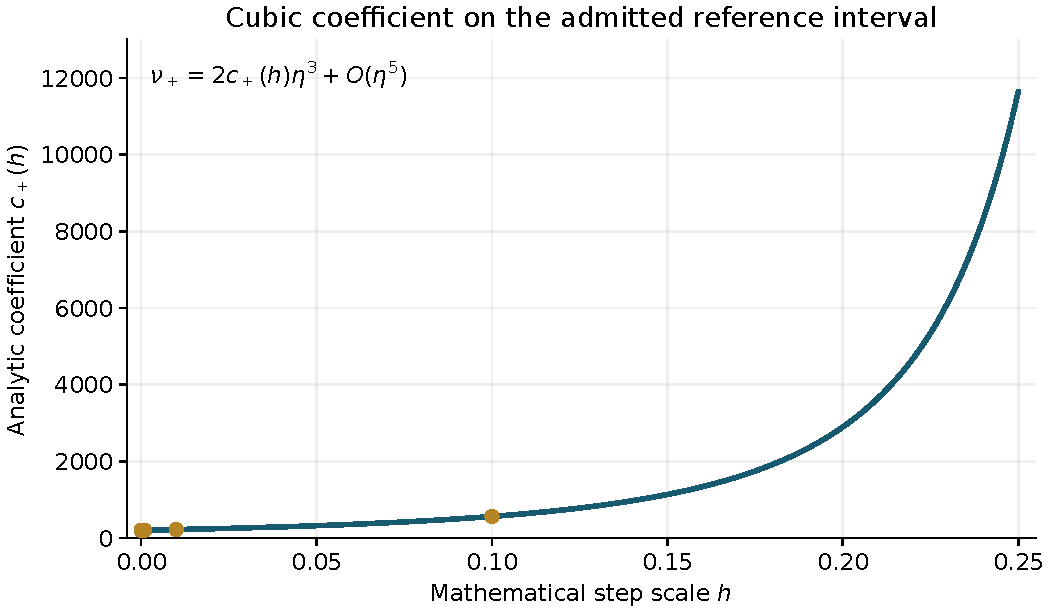
\includegraphics[width=.82\textwidth]{figures/coefficient.pdf}\caption{Evaluation of the proved \(c_+(h)\) formula (D3) on \(0\le h\le1/4\). Dots identify the four retained certificate step values; they evaluate the analytic coefficient, not finite-\(\eta\) rates or newly certified fixtures. The axis \(h\) is a mathematical step scale. Figure code and formula samples are supplied.}\label{fig:coefficient}\end{figure}

\section{Necessary drift identities and their meaning}

The prestage is \(A_k(z)=B(z)z\), with real symmetric
\[
B(z)=\operatorname{diag}[1+\epsilon(k_i-|z_i|^2)]+g\Delta.
\]

Therefore \(z^\dagger A_k(z)\) is real. At a relative equilibrium the synchronizer preserves each modulus, so
\(\widetilde z_i=e^{i(\omega-\delta_i)}z_i\). Taking the imaginary part proves the exact finite-step identity

\[
\boxed{\sum_i|z_i|^2\sin(h\nu-\delta_i)=0,}
\tag{D39}\label{eq:D39}
\]

where the kicks use the actual prestage. Setting \(S_\delta=\sum_i|z_i|^2e^{i\delta_i}\) gives \(\omega=\arg S_\delta\pmod\pi\) \textbf{only when \(S_\delta\ne0\)}. Otherwise the sine identity imposes no angle restriction. The selected small-step domain excludes this issue: \(|\delta_i|\le2|\lambda|\le1/60\) gives \(\Re S_\delta>0\).

At a generator relative equilibrium \(X_k(z)=i\nu z\), the onsite/\allowbreak{}coupling part again has real total pairing. Hence, with \(z_i=r_i e^{i\theta_i}\),

\[
\boxed{\nu\sum_i r_i^2=\frac1{30}\sum_i r_i^2
\sum_{j\ne i}\sin3(\theta_j-\theta_i)
=\frac1{30}\sum_{i<j}(r_i^2-r_j^2)\sin3(\theta_j-\theta_i).}
\tag{D40}\label{eq:D40}
\]

The final equality pairs opposite orientations and keeps the \textbf{positive} \(1/30\) sign. Unweighted kicks cancel pairwise, but unequal amplitude weights leave a possible net contribution. D1 finds it after solving amplitudes and phase differences together. This is an explanation of the established solution's balance, not an existence proof by itself.

The finite-step sine identity and the generator identity must remain distinct. At finite step, zero total kick alone does not make the argument of its exponential sum vanish: \(2e^{it}+e^{-2it}\) generically has nonzero imaginary part despite kicks summing to zero. Thus a leading small-kick correlation formula is not an all-orders necessity theorem for finite-step amplitude inhomogeneity. [D0 \S{}5; D1 \S{}7; closeout \S{}4 and local record.]

\section{What the interval certificates prove}

\textbf{Retained validated numerical result.} The finite coverage is exactly

\[
h\in\{0,1/10,1/100,1/1000\},\qquad
\eta\in\{\pm1/1000,\pm1/2000,\pm1/4000\}.
\tag{D41}\label{eq:D41}
\]

The original proposed ladder \(\pm1/100,\pm1/200,\pm1/400\) was not certified. With a fixed 64-subinterval path budget, the first interval at \(h=1/10\), \([0,(1/100)/64]\), had contraction bound above 4.077. That failure is a failure of a sufficient enclosure, not evidence of nonexistence or a bifurcation. The entire nested ladder was reduced tenfold without changing hatted coefficients, mean, direction, gauge or branch.

The distinction between approximation and mathematical verification is standard \cite{Rump}. That reference supplies context for enclosure methods, not an audit of this implementation.

D1 uses 110-digit Newton approximations followed by 100-digit outward-rounded interval arithmetic. Precision alone does not prove a root. For parameter interval \(E\), centre \(x_c\in\mathbb R^7\), box \(X=x_c+[-r,r]^7\), and fixed approximate inverse \(C\), the certificates bound the complete derivative:

\[
Y\ge\sup_{\eta\in E}\|CG(x_c,\eta)\|_\infty,\qquad
q_{\rm ctr}\ge\sup_{x\in X,\eta\in E}\|I-CG_x(x,\eta)\|_\infty.
\]

\[
\boxed{q_{\rm ctr}<1,\qquad Y+q_{\rm ctr}r<r.}
\tag{D42}\label{eq:D42}
\]

Then \(x\mapsto x-CG(x,\eta)\) is a contraction into the interior of \(X\) for every \(\eta\in E\). Banach's theorem proves a unique root in the box and nonsingularity, with
\(\|G_x^{-1}\|_\infty\le\|C\|_\infty/(1-q_{\rm ctr})\).
The inverse need only be approximate; the norm inequality proves the required invertibility.

The positive path \([0,1/1000]\) is divided into 64 intervals at each \(h\), giving \textbf{256 parameter boxes}. At their endpoints, \textbf{260} additional radius-\(10^{-60}\) root boxes are enclosed in the adjacent parameter boxes. The endpoint root is therefore the same unique root from either side; the first contains the exact D0 reference. This proves connection, not merely a sequence of small residuals. Negative-\(\eta\) paths follow by conjugation composed with \(j\mapsto2-j\), with extra fixed-root checks; conjugation transports the proof to negative chirality.

The removable quotient in \eqref{eq:D34} uses its entire series through degree 24 with rigorous tail
\[
\left|E_h(t)-\sum_{n=1}^{24}\frac{-(-i)^n h^{n-1}t^n}{n!}\right|
\le\frac{|h|^{24}|t|^{25}e^{|ht|}}{25!}.
\tag{D43}\label{eq:D43}
\]

Its real/\allowbreak{}imaginary derivatives are \(\sin(ht)\) and \(\cos(ht)\); at \(h=0\) the formula is exactly \(it\). Positive modulus bounds justify all denominators and square roots.

\begingroup\small\setlength{\LTpre}{5pt}\setlength{\LTpost}{7pt}
\begin{longtable}{@{}>{\raggedright\arraybackslash}p{0.1000\dimexpr\textwidth-48pt\relax}>{\raggedright\arraybackslash}p{0.2100\dimexpr\textwidth-48pt\relax}>{\raggedright\arraybackslash}p{0.2300\dimexpr\textwidth-48pt\relax}>{\raggedright\arraybackslash}p{0.2300\dimexpr\textwidth-48pt\relax}>{\raggedright\arraybackslash}p{0.2300\dimexpr\textwidth-48pt\relax}@{}}
\toprule
\textbf{\(h\)} & \textbf{Maximum \(q_{\rm ctr}\) below} & \textbf{Minimum input modulus squared above} & \textbf{Minimum prestage modulus squared above} & \textbf{Border inverse norm below}\\ \midrule
\endfirsthead
\textbf{\(h\)} & \textbf{Maximum \(q_{\rm ctr}\) below} & \textbf{Minimum input modulus squared above} & \textbf{Minimum prestage modulus squared above} & \textbf{Border inverse norm below}\\ \midrule
\endhead
\bottomrule\endfoot
0 & 0.196109 & 0.497619 & 0.497619 & 72.417\\[4pt]
1/\allowbreak{}10 & 0.523617 & 0.495978 & 0.495886 & 189.991\\[4pt]
1/\allowbreak{}100 & 0.212847 & 0.497508 & 0.497501 & 76.597\\[4pt]
1/\allowbreak{}1000 & 0.197700 & 0.497608 & 0.497608 & 72.811\\[4pt]
\end{longtable}\endgroup

These are the report's deliberately weakened outward bounds for the normalized full system, not condition numbers in arbitrary coordinates. D1 gives a conservative factor-two conversion for the original real infinity norm. Gauge positivity and phase deviation below 0.016566 radians keep the winding and chirality labels fixed along the paths. No trajectory was used. [D1 \S{}5.]

\subsection{Rates, coefficient comparison, and control}

There are 24 independently isolated positive-chirality points, including both signs of \(\eta\), and their exact conjugates: 48 accepted chiral-root records. Each rate coordinate has certified error at most \(10^{-60}\). Representative \textbf{rounded midpoint values} at the smallest positive \(\eta=1/4000\) are:

\begingroup\small\setlength{\LTpre}{5pt}\setlength{\LTpost}{7pt}
\begin{longtable}{@{}>{\raggedright\arraybackslash}p{0.2500\dimexpr\textwidth-36pt\relax}>{\raggedright\arraybackslash}p{0.2400\dimexpr\textwidth-36pt\relax}>{\raggedright\arraybackslash}p{0.2700\dimexpr\textwidth-36pt\relax}>{\raggedright\arraybackslash}p{0.2400\dimexpr\textwidth-36pt\relax}@{}}
\toprule
\textbf{\(h\)} & \textbf{\(\nu_+\)} & \textbf{\(\nu_+/(2\eta^3)\)} & \textbf{Exact \(c_+(h)\), rounded}\\ \midrule
\endfirsthead
\textbf{\(h\)} & \textbf{\(\nu_+\)} & \textbf{\(\nu_+/(2\eta^3)\)} & \textbf{Exact \(c_+(h)\), rounded}\\ \midrule
\endhead
\bottomrule\endfoot
0 & \(6.20618242410550\,10^{-9}\) & 198.59783757138 & 198.60849260123\\[4pt]
1/\allowbreak{}10 & \(1.74764433349168\,10^{-8}\) & 559.24618671734 & 559.11239698359\\[4pt]
1/\allowbreak{}100 & \(6.77634944420660\,10^{-9}\) & 216.84318221461 & 216.85381829653\\[4pt]
1/\allowbreak{}1000 & \(6.26019299725693\,10^{-9}\) & 200.32617591222 & 200.33684804178\\[4pt]
\end{longtable}\endgroup

The complete twelve-positive-point table and both signs/\allowbreak{}labels remain in D1 \S{}6 and its results. Finite ratios are not exact coefficients. Root uncertainty contributes at most \(10^{-60}/(2|\eta|^3)\le3.2\,10^{-50}\); truncation effects are much larger. Analyticity proves
\[
\nu_+/(2\eta^3)-c_+(h)=O(\eta^2).
\tag{D44}\label{eq:D44}
\]
The recorded enclosures of that difference divided by \(\eta^2\) have magnitude below \(2.141\,10^6\) \textbf{at the twelve positive fixtures}. They are not an explicit uniform remainder bound between them.

The separate control uses \(h=1/10,\eta=1/100000,\kappa=(1,1,-2)\), with a connected parameter box \(q_{\rm ctr}<0.372566\) and an endpoint root box. The equal-coefficient reflection combined with conjugation preserves this local branch and reverses its rate. Uniqueness therefore gives \(\nu=0\) exactly. Its approximate rate \(-1.17\,10^{-116}\) is rounding residue.

Absolute original real residual components over the fixed-root boxes are at most \(2.84\,10^{-60}\), and absolute identity residual components are at most \(2.16\,10^{-60}\). At the enclosed exact root the equations vanish exactly. Independent 110-digit midpoint identities below \(2.32\,10^{-108}\), and native complex128 relative-equilibrium discrepancies below \(3.15\,10^{-16}\), are supporting diagnostics, not substitutes for \eqref{eq:D42}. [D1 \S{}\S{}6--8.]

\section{State advance and stationary invariant observations}

At a relative equilibrium,
\[
z^+=e^{i\omega}z\quad\Longrightarrow\quad
\boxed{z^+(z^+)^\dagger=zz^\dagger.}
\tag{D45}\label{eq:D45}
\]

The scalar phase cancels its conjugate. Thus every component intensity, pair coherence, winding and already defined common-phase-invariant chirality readout stays fixed. At \(X=i\nu z\), differentiation of \(zz^\dagger\) gives \(i\nu zz^\dagger-i\nu zz^\dagger=0\).

For the raw channel chirality \(C=\Re z\times\Im z\), a common phase rotates the two real channel vectors by an \(SO(2)\) matrix; their cross product is unchanged. This is also visible from the imaginary parts of the pair coherences. It is an inherited observable identity, not a conservation law for arbitrary native trajectories. D0 supplies a simple counterexample to general conservation: with \(g=\lambda=0,\epsilon=1/4,k=0\), a state whose component moduli all equal one is multiplied by \(3/4\), so its nonzero chirality is multiplied by \(9/16\).

Consequently the full state advances on a group orbit while its coherence quotient is stationary. This does not declare common phase physically unobservable, nor say that every possible readout ignores it. It supplies no map from phase to core position, ambient rotation, a moving measurement cylinder, or a physical current. [Native readouts.py; D0 \S{}\S{}3,5; D1 \S{}7; closeout \S{}6.]

\section{The accepted conditional pure-gradient obstruction}

The written closeout adds a precise consequence at the generator level. Suppose, on a domain containing the established nonzero-rate states,
\[
X=-\operatorname{grad}_{g_*}V,\qquad g_*>0,\qquad
V(e^{i\alpha}z)=V(z),
\tag{D46}\label{eq:D46}
\]
where \(V\) is differentiable and \(g_*\) is positive definite. The metric need not itself be phase-invariant for this argument.

At a nonzero relative equilibrium \(X=i\nu z\), \(\nu\ne0\), invariance gives
\[
dV(X)=\nu\,dV(iz)=0.
\]
But the gradient representation requires
\[
dV(X)=-g_*(\operatorname{grad}_{g_*}V,
\operatorname{grad}_{g_*}V)<0,
\tag{D47}\label{eq:D47}
\]
because \(X\ne0\). This contradiction rules out that specified \textbf{single invariant-potential pure-gradient representation}.

This is a conditional exact argument retained from closeout, not a statement that every dynamical description is excluded. It does not classify non-gradient, indefinite-metric, driven, Hamiltonian or other representations; it does not turn the finite map into a flow. In particular it does not conflict with the two separate increment identities \eqref{eq:D9} and \eqref{eq:D11}. [Supplied closeout \S{}5; local closeout \textquotedblleft{}Review consequences.\textquotedblright{}]

\section{Conclusions and limits}

D0 makes the nonlinear question well posed by providing a regular chiral saddle reference and an invertible seven-variable border, including the desingularized generator endpoint. Symmetry allows a cubic rate and excludes the quartic term; D1's complete state calculation supplies the missing nonzero coefficient. Connected interval certificates establish finite roots on the exact retained ladder. The weighted identities explain the resulting phase balance, while coherence invariance explains why selected passive readouts remain stationary.

The accepted result is a native common \textbf{complex-phase} advance, local to this branch and family. It does not certify attraction, arbitrary unequal coefficients, broader rings, a calibrated physical frequency or spatial motion. The formal step scale remains mathematical. This publication presents the established result; it adds no continuation beyond D1.

\clearpage\appendix
\section{Full implicit-series state corrections}

The following are D1 \S{}3's complete coefficients in \eqref{eq:D31}, retained for a checkable coefficient proof. Set \(d_h=3h-1\) and

\[
\begin{aligned}
P_h&=108h^3+27h^2+828h-760,\\
Q_h&=54h^3-270h^2-261h+592,\\
U_h&=972h^5+2025h^4+12744h^3+96570h^2+132h+64568,\\
W_h&=972h^5-8667h^4+112212h^3-521514h^2+98412h-206440.
\end{aligned}\tag{DA1}\label{eq:DA1}
\]

Using \(u=\sum_{n=1}^3\eta^n u_n+O(\eta^4)\), \(v=\sum_{n=1}^3\eta^n v_n+O(\eta^4)\), the order-one coefficients are

\[
u_1=-\frac{3h+2}{d_h}(1,0,-1),\qquad
v_1=\frac{\sqrt3(3h-10)}{3d_h}(1,-2,1).
\tag{DA2}\label{eq:DA2}
\]

The second-order coefficients are

\[
u_2=-\frac{P_h}{6d_h^3}(1,0,1)
-\frac{Q_h}{3d_h^3}(0,1,0),\qquad
v_2=-\frac{\sqrt3(3h-10)(45h-68)}{2d_h^3}(1,0,-1).
\tag{DA3}\label{eq:DA3}
\]

The third-order coefficients are

\[
u_3=-\frac{U_h}{6d_h^5}(1,0,-1),\qquad
v_3=\frac{\sqrt3 W_h}{18d_h^5}(1,-2,1),
\tag{DA4}\label{eq:DA4}
\]

\[
\nu_1=\nu_2=0,\qquad
\nu_3=-\frac{\sqrt3(33h^2-240h+688)}{3d_h^3}.
\tag{DA5}\label{eq:DA5}
\]

Each \(v_n\) has zero sum, as required by the gauge. Both real and imaginary state coordinates change; no fixed-amplitude ansatz is used. The normalized border has phase column \((0,0,0,-1,-1,-1)^T\) and gauge row \((0,0,0,1/3,1/3,1/3)\), with the same determinant \eqref{eq:D25}.

To see the exact verification logic, write \(p_i=1+\eta p_{i1}+\eta^2p_{i2}+\eta^3p_{i3}+\cdots\) from \eqref{eq:D32}, and \(|p_i|^2=1+s_i\). Use
\[
(1+s_i)^{-3/2}=1-\frac32s_i+\frac{15}{8}s_i^2-\frac{35}{16}s_i^3+O(\eta^4).
\tag{DA6}\label{eq:DA6}
\]
Multiplication by \(p_i^3\) gives \(C_i\). Form the imaginary products in \eqref{eq:D33}, expand the two exponentials, and collect powers of \(\eta\) in all six real equations and the gauge. At each order, the coefficient of the new state/\allowbreak{}rate vector is the same full reference derivative; all other terms are the already determined forcing in \eqref{eq:D35}. D1 solves these three exact linear systems, then substitutes the complete result again into the original residual. The stored exact\_\allowbreak{}jet records the 21 solved real coefficients and zero residual coefficients. This derivation and substitution, together with isolation, are the coefficient proof; 110-digit residual scaling is only a separate check.

\section{Scientific corrections and source record}

The determinant placement, reflection action, gradient qualifications and zero-domain restrictions are retained in the arguments above. The original correction table is retained in the provenance record. The public master derivative preserves its scientific content; the raw original remains privately archived. Current receipt of reviewer companions is recorded below.

\section{Notation, source ownership, and evidence}

\begingroup\small\setlength{\LTpre}{5pt}\setlength{\LTpost}{7pt}
\begin{longtable}{@{}>{\raggedright\arraybackslash}p{0.2500\dimexpr\textwidth-24pt\relax}>{\raggedright\arraybackslash}p{0.3700\dimexpr\textwidth-24pt\relax}>{\raggedright\arraybackslash}p{0.3800\dimexpr\textwidth-24pt\relax}@{}}
\toprule
\textbf{This text} & \textbf{Source symbol or convention} & \textbf{Meaning}\\ \midrule
\endfirsthead
\textbf{This text} & \textbf{Source symbol or convention} & \textbf{Meaning}\\ \midrule
\endhead
\bottomrule\endfoot
\(z\) & Native \(\Omega\); D0/\allowbreak{}D1 \(z\) & Canonical complex state, not spatial position\\[4pt]
\(h,\nu,\omega\) & D0/\allowbreak{}D1 unchanged & Mathematical step scale, rescaled rate, per-step angle\\[4pt]
\(\lambda,\ell=3\lambda\) & Native phase\_\allowbreak{}strength, D0/\allowbreak{}D1 \(\ell\) & Phase coefficient and harmonic derivative coefficient\\[4pt]
\(\mathcal V,\mathcal E\) & D0 \(V,E\) & Quartic state potential and fixed phase energy\\[4pt]
\(R,H,P\) in \S{}4 & NRG/\allowbreak{}D0 response matrices & Background diagonal, Cartesian pre-block, phase pre-block; not scaffold lengths\\[4pt]
\(V_r,\chi_r,\Gamma_r\) & D0 \S{}3 \(V,\chi,\Gamma\) & Response obstruction factors; \(\Gamma_z\) is state chirality\\[4pt]
\(\mathcal A(x)\) & D0 \S{}8 \(V(x)\) & Oriented Vandermonde \((x_0-x_1)(x_1-x_2)(x_2-x_0)\)\\[4pt]
\(q_\phi\), \(q_h\), \(q_{\rm ctr}\) & D0 group tangent \(q\), polynomial \(q_h\); D1 contraction \(q\) & Three different objects, explicitly distinguished\\[4pt]
\(q_j\) & D1 \(q_j=e^{2\pi ij/3}\) & Reference root of unity; not the lens ratio in the companion text\\[4pt]
\(d_h,P_h,Q_h,U_h,W_h\) & D1 \(d,P,Q,U,W\) & Jet polynomials; distinct from kicks \(\delta_i=hd_i\)\\[4pt]
\(g_*\) & Closeout metric \(g\) & Positive-definite metric in the conditional obstruction, not graph coupling\\[4pt]
\end{longtable}\endgroup

\begingroup\small\setlength{\LTpre}{5pt}\setlength{\LTpost}{7pt}
\begin{longtable}{@{}>{\raggedright\arraybackslash}p{0.2500\dimexpr\textwidth-24pt\relax}>{\raggedright\arraybackslash}p{0.3700\dimexpr\textwidth-24pt\relax}>{\raggedright\arraybackslash}p{0.3800\dimexpr\textwidth-24pt\relax}@{}}
\toprule
\textbf{Claim/\allowbreak{}equations} & \textbf{Supporting source location} & \textbf{Evidence/\allowbreak{}ownership}\\ \midrule
\endfirsthead
\textbf{Claim/\allowbreak{}equations} & \textbf{Supporting source location} & \textbf{Evidence/\allowbreak{}ownership}\\ \midrule
\endhead
\bottomrule\endfoot
Ordered map, regular domain: D5--D7 & \href{\detokenize{supplement/historical/D0_chiral_reference_20261006/D0_CHIRAL_REFERENCE_AND_RECONCILIATION.md}}{D0} \S{}2, \S{}4.3; native dynamics.py 57--112 & Inherited Paper A definition; checked domain qualification\\[4pt]
Gradient identities/\allowbreak{}descent: D8--D11 & D0 \S{}4; native z\_\allowbreak{}diagnostics.py potential; inherited GR0/\allowbreak{}NRG & Derived identities and conditional inequalities\\[4pt]
Weights and diagonal versus SPD balance: D12--D14 & \href{\detokenize{supplement/historical/project/NATIVE_RESPONSE_GEOMETRY/manuscript/response.tex}}{NRG response manuscript}, weighted response/\allowbreak{}cycle sections; \href{\detokenize{supplement/historical/project/NATIVE_RESPONSE_GEOMETRY/manuscript/spectral.tex}}{NRG spectral manuscript}, SPD criterion; D0 \S{}4.3 & Prior accepted response results, not new D1 claims\\[4pt]
Coefficient-placement correction: D15--D18 & D0 \S{}3; original review script Sections B/\allowbreak{}F & Exact Laurent identities and characteristic shifts\\[4pt]
Reference, complete derivative, saddle: D19--D22 & D0 \S{}\S{}6--7 & Exact native ansatz and full mixed Jacobian\\[4pt]
Gauge, border, extension: D23--D27 & D0 \S{}\S{}7.1--7.2 & Exact determinant; analytic implicit-function theorem\\[4pt]
Joint symmetries/\allowbreak{}divisibility: D28--D30 & D0 \S{}\S{}5,8; \href{\detokenize{supplement/historical/FRESH_EYES_SCIENTIFIC_REVIEW_20261006/FRESH_EYES_RECONCILIATION_NOTE_v0.1.md}}{reconciliation} \S{}\S{}3.2--3.3 & Exact theorem with local uniqueness hypotheses\\[4pt]
Native jet/\allowbreak{}coefficient: D31--D38, DA1--DA6 & \href{\detokenize{supplement/historical/D1_chiral_drift_20261006/D1_NATIVE_CHIRAL_PHASE_DRIFT.md}}{D1} \S{}\S{}2--4; verify\_\allowbreak{}d1.py jet\_\allowbreak{}residual/\allowbreak{}derive\_\allowbreak{}jets; results exact\_\allowbreak{}jet & Exact derivation/\allowbreak{}substitution; analytic asymptotics\\[4pt]
Drift balance: D39--D40 & D0 \S{}5; D1 \S{}7; \href{\detokenize{supplement/reviewer/D1_GPT_REVIEW/D1_SCIENTIFIC_CLOSEOUT.md}}{closeout} \S{}4 & Necessary identities, distinct from existence proof\\[4pt]
Finite certificates: D41--D44 & D1 \S{}\S{}5--6; \href{\detokenize{supplement/historical/D1_chiral_drift_20261006/D1_RESULTS.json}}{original results}, continuation\_\allowbreak{}tubes/\allowbreak{}continuation\_\allowbreak{}endpoints/\allowbreak{}roots\_\allowbreak{}plus/\allowbreak{}roots\_\allowbreak{}minus/\allowbreak{}two\_\allowbreak{}equal\_\allowbreak{}control/\allowbreak{}interval\_\allowbreak{}summary & Retained validated numerics versus midpoint diagnostics\\[4pt]
Invariant observations: D45 & D1 \S{}7; closeout \S{}6; native readouts.py & Exact identity; inherited passive observables\\[4pt]
Conditional pure-gradient obstruction: D46--D47 & Closeout \S{}5; \href{\detokenize{supplement/historical/D1_scientific_closeout_20261006/D1_LOCAL_CLOSEOUT_RECORD.md}}{local closeout record}, \textquotedblleft{}Review consequences\textquotedblright{} & Accepted conditional contradiction proof\\[4pt]
\end{longtable}\endgroup

The inherited recurrence predates D0/\allowbreak{}D1. NRG already owns the retained response classification and spatial/\allowbreak{}attachment distinctions; Paper G already studies the raw/\allowbreak{}attached chirality framework and its separate dynamical results. This text makes no novelty claim or revision of either publication.

\subsection{Counts and reproducibility boundaries}

\begingroup\small\setlength{\LTpre}{5pt}\setlength{\LTpost}{7pt}
\begin{longtable}{@{}>{\raggedright\arraybackslash}p{0.2500\dimexpr\textwidth-24pt\relax}>{\raggedright\arraybackslash}p{0.3700\dimexpr\textwidth-24pt\relax}>{\raggedright\arraybackslash}p{0.3800\dimexpr\textwidth-24pt\relax}@{}}
\toprule
\textbf{Checkpoint} & \textbf{Recorded result} & \textbf{Categories, unchanged}\\ \midrule
\endfirsthead
\textbf{Checkpoint} & \textbf{Recorded result} & \textbf{Categories, unchanged}\\ \midrule
\endhead
\bottomrule\endfoot
D0 & \textbf{64/\allowbreak{}64} & 36 exact symbolic; 11 numerical evidence; 2 native numerical; 11 preservation; 4 source/\allowbreak{}byte\\[4pt]
D1 & \textbf{133/\allowbreak{}133} & 8 exact symbolic; 57 validated numerical; 53 unvalidated numerical; 11 preservation; 4 source/\allowbreak{}byte\\[4pt]
\end{longtable}\endgroup

These are named heterogeneous predicates, not independent-theorem counts. No review printout or reviewer-companion check is added to either total. NRG's \textbf{61} paper-local checks and its \textbf{429} retained checkpoint checks remain separate prior records, not D0/\allowbreak{}D1 counts.

The D1 certificate set establishes the ideal mathematical equations with its recorded arithmetic and domains; binary64 comparisons are a different evidence class. Reviewer companions are now included with verified archival hashes. Their stored outcomes remain retained review evidence, not newly reproduced certificates or an audit of D1's interval implementation. The reviewed master consolidation performed editorial/\allowbreak{}source checks only; the publication package retains and repeats the bounded portable smoke path documented in the joint build record.

\section*{Acknowledgments and AI-assistance disclosure}
The author acknowledges assistance from ChatGPT/GPT in scientific review and work-order preparation, and from Codex in explanatory organization, transcription, packaging, typesetting and bounded checks. These contributions do not constitute external peer review or independent certification. Assertions are supported by written arguments and specifically identified evidence.
\clearpage
\section*{Code and evidence availability}
The source project is \url{https://github.com/pzychozen/trioctagon-physics}. Scientific definitions use the unchanged baseline commit \texttt{82cab10cbe550f58c43163fb8b05fabdad1b05ae}.
The planned publication-package location is \path{papers/MEASUREMENT_AND_CHIRAL_DRIFT/v0.1/} in that repository. These final files are prepared; repository publication is pending. The shared package contains two separate papers, their sources, figures and supporting evidence.

The complete extracted package provides the local supplement links used here. Its source inventory and public-export map distinguish unchanged copies from labeled public derivatives, retain both raw-original and public-file hashes, and specify exact operational omissions and locator substitutions. Scientific data are preserved; private raw records remain separately archived.
The joint README documents bounded build and smoke commands using the pinned native subset and unchanged verifier function bodies. Historical writers must not be executed in-place; the active tools use designated output records. Full historical suites and reviewer companion scripts were not regenerated. Retained evidence, prior review receipts and final packaging checks remain separate.

The five reviewer companion files are included with their received hashes; the original ZIP identity is retained in provenance. They were unavailable during the earlier local closeout; that historical statement is preserved. The scripts and stored outputs are reviewer companions, not an audit of D1's interval verifier. No companion-script replay is claimed here.

The software subset retains its original Apache-2.0 license and scope notice. That license is not assigned to manuscripts, research scripts, results or figures. This packaging grants no new redistribution rights and claims no external peer review, journal acceptance or DOI.

\clearpage

\begin{thebibliography}{99}
\bibitem{TL} H. F. Halldórsson, TL0--TL4 measurement and lens-interface research checkpoints (2026). Public reports, verifier-source derivatives and retained scientific results in the measurement supplement; original and public hashes in the source inventory.
\bibitem{D0D1} H. F. Halldórsson, D0: Chiral Reference and Reconciliation; D1: Native Chiral Phase Drift, and supplied scientific closeout (2026). Reports and evidence in the drift supplement.
\bibitem{native} Tri-Octagon scientific project, \texttt{kernel\_physics} definitions, pinned revision \texttt{82cab10cbe550f58c43163fb8b05fabdad1b05ae} (2026). Native subset, original software license and scope notice.
\bibitem{NRG} H. F. Halldórsson, \emph{Native Response Geometry and Spectral Circulation in the Tri-Octagon Map}, research publication v0.1 (2026). Prior response classification; manuscript sources in the drift supplement.
\bibitem{PaperA} H. F. Halldórsson, \emph{Cycle-Covering Dynamics of a Three-State Nonlinear Kernel}, Paper A project manuscript v0.5.1 (2026). Inherited recurrence; retained source in the drift supplement.
\bibitem{PaperG} Tri-Octagon research programme, Paper G project record (2026). Prior chirality framework; source locator and status in the supplement.

\bibitem{AK} I. S. Aranson and L. Kramer, The world of the complex Ginzburg--Landau equation, \emph{Reviews of Modern Physics} 74 (2002), 99--143. \href{https://doi.org/10.1103/RevModPhys.74.99}{doi:10.1103/RevModPhys.74.99}. \href{https://arxiv.org/abs/cond-mat/0106115}{Author preprint}, Section II.A, equations (7)--(9).
\bibitem{PAL} F. C. Poderoso, J. J. Arenzon and Y. Levin, New ordered phases in a class of generalized XY models, \emph{Physical Review Letters} 106 (2011), 067202. \href{https://doi.org/10.1103/PhysRevLett.106.067202}{doi:10.1103/PhysRevLett.106.067202}. \href{https://arxiv.org/abs/1008.0868}{Author preprint}, equation (1).
\bibitem{Krupa} M. Krupa, Bifurcations of Relative Equilibria, \emph{SIAM Journal on Mathematical Analysis} 21(6) (1990), 1453--1486. \href{https://doi.org/10.1137/0521081}{doi:10.1137/0521081}.
\bibitem{Rump} S. M. Rump, Verification methods: rigorous results using floating-point arithmetic, \emph{Acta Numerica} 19 (2010), 287--449. \href{https://doi.org/10.1017/S096249291000005X}{doi:10.1017/S096249291000005X}. \href{https://www.tuhh.de/ti3/rump/intlab/ActaNumerica2010.pdf}{Author manuscript}, Sections 1.1--1.4 and 13.1, Theorem 13.3.

\end{thebibliography}

\end{document}
